\chapter{Umsetzung des Prototypen}

Die Umsetzung des Prototypen entspricht dem Hauptteil dieser Arbeit. Wie eingehend beschrieben, soll ein Prototyp entwickelt werden, der die Montage von Rauchmeldern in einer augmentierten Umgebung visualisiert. Dabei sollen Smartphones und Tablets sowohl als Ausgabegeräte als auch als Eingabegeräte verwendet werden. Im Folgenden wird die Umsetzung des Prototypen, die sowohl die Konzeption als auch die Implementierung  und die Beschreibung der Anforderungen umfasst, dargestellt.

\section{Anforderungen}

- Framework für die Montageregeln

Damit der Prototyp zielgerichtet entwickelt werden kann, müssen zunächst die Anforderungen definiert werden. Diese Anforderungen bilden die Grundlage für die weitere Konzeption und Implementierung des Anwendung. Dazu wurden verschiedenste Einflussfaktoren berücksichtigt, die die Anforderungen an das System beeinflussen.

\subsection{Benutzerinteraktion}

Die Implementierung von Interaktionen in Augmented-Reality-Anwendungen muss sorgfältig geplant werden, um eine intuitive Bedienung zu gewährleisten. Die Interaktionen sollten einfach und schnell durchführbar sein, um den Benutzer nicht zu überfordern. Der Benutzer sollte sofort erkennen können, wie er mit der Anwendung interagieren kann. 

Es ist eine Reihe von Interaktionen denkbar, die dem Benutzer die Möglichkeit geben, mit der augmentierten Umgebung zu interagieren. Dazu gehören beispielsweise Handgesten vor der Kamera, Sprachbefehle oder Touch-Gesten. 

Aufgrund des Einsatzes von Smartphones und Tablets sind die Interaktionsmöglichkeiten jedoch begrenzt. Dies liegt vor allem daran, dass das Ausgabegerät während der Nutzung in der Hand gehalten werden muss. Bei der Verwendung von Tablets müssen je nach Größe des Gerätes sogar beide Hände verwendet werden, um das Gerät stabil halten zu können. Unter der Annahme, dass das Tablet wie in Abbildung \ref{fig:ipad} gehalten wird, sind die Interaktionsmöglichkeiten auf die Daumen des Benutzers und die Ausrichtung bzw. Position des Gerätes beschränkt. Die Bedienungsmöglichkeiten der AR-Anwendung sollten aus diesem Grund so einfach und minimal wie möglich gehalten werden, sodass der Benutzer die Anwendung bedienen kann ohne, dass die Gefahr besteht, das Gerät fallen zu lassen.

\subsection{Genauigkeit}

Die Visualisierung von Montageregeln für Rauchmelder erfordert eine hohe Genauigkeit bei der Tiefenmessung und dem Tracking der Umgebung. Wie einleitend beschrieben, können ungenaue Montagen von Rauchmeldern fatale Folgen haben. Aus diesem Grund ist es wichtig, sicher zu stellen, dass die Dimensionen des Weltkoordinatensystems, in dem die Rauchmelder platziert werden, mit der realen Welt übereinstimmen. Nur so kann sichergestellt werden, dass Abstände korrekt gemessen und Rauchmelder korrekt platziert werden können.

\subsection{Echtzeitdarstellung}

Die Echtzeitdarstellung ist ein wichtiger Bestandteil von Augmented-Reality-Anwendungen, da sie maßgeblich zum Benutzererlebnis beiträgt. Dabei ist es wichtig Latenzen und Drift-Effekte, also die Abweichung der virtuellen Objekte von ihrer tatsächlichen Position, zu minimieren. Es ist demnach sicherzustellen, dass die Verarbeitung der Sensordaten und die Darstellung bzw. Positionierung der virtuellen Objekte möglichst performant implementiert werden und sich nicht gegenseitig blockieren. Auch Benutzerinteraktionen sollten nicht zu Verzögerungen führen, da dies das Benutzererlebnis negativ beeinflussen würde.

\subsection{Feedback}

Feedback ist ein wichtiger Bestandteil von Augmented-Reality-Anwendungen. AR-Systeme können je nach Status des Tracking-Zustands abweichende beziehungsweise unerwartete Ergebnisse liefern. Es ist daher wichtig, dem Benutzer Feedback zu geben, um ihn über den aktuellen Status der Anwendung zu informieren. 

Zusätzlich ist es wichtig, den Benutzer auf Fehlverhalten hinzuweisen, um ihm die Möglichkeit zu geben, dieses zu korrigieren. Dies kann beispielsweise durch visuelle Hinweise oder Textnachrichten geschehen.

\subsection{Verzicht auf manuelle Kalibrierung und Initialisierung}

Falls die Anwendung in einem professionellen Umfeld eingesetzt werden soll, ist es wichtig, dass die Anwendung eine möglichst geringe Einstiegshürde aufweist. Dies bedeutet, dass die Anwendung ohne manuelle Kalibrierung oder Initialisierung starten sollte. Der Benutzer sollte die Anwendung starten und sofort mit der Interaktion beginnen können. Dies ist besonders wichtig, wenn die Anwendung in einem professionellen Umfeld eingesetzt wird, in dem Zeit ein kritischer Faktor ist.

\section{Konzeption}

Das Konzept des Prototypen wurde iterativ entwickelt und nicht in einem einzigen Schritt abgeschlossen. Dabei wurden die Lösungsansätze zur Umsetzung der Anforderungen schrittweise umgesetzt und verfeinert.

Im ersten Schritt wurde eine grundlegende Skizze des Prototypen erstellt (siehe Abbildung \ref{fig:Concept}), die die wichtigsten Funktionen und Interaktionen darstellte. Diese Skizze diente als Ausgangspunkt für die weitere Entwicklung.

Die Hauptkomponenten des Konzepts umfassen:

\begin{itemize}
    \item \textbf{Anzeige von Flächen:} Die Anwendung soll in der Lage sein, Flächen in der Umgebung zu erkennen und anzuzeigen.
    \item \textbf{Darstellung der Montageregeln:} Die Montageregeln sollen direkt an der Decke in Form von Farbflächen dargestellt werden.
    \item \textbf{Automatische Platzierung eines virtuellen Rauchmelders:} Der Prototyp soll, basierend auf den erkannten Flächen und den Montageregeln, in der Lage sein, einen virtuellen Rauchmelder automatisch an die optimale Position zu platzieren.
    \item \textbf{Darstellung des Rauchmelders:} Die Rauchmelder sollen in der augmentierten Umgebung dargestellt werden, um dem Benutzer eine genaue Vorstellung von deren Position zu geben.
    \item \textbf{Distanzindikatoren:} Um sicherzustellen, dass die Rauchmelder korrekt platziert werden, sollen Distanzindikatoren verwendet werden, die dem Benutzer die Abstände anzeigen.
    \item \textbf{Informationsanzeige:} Die Anwendung soll dem Benutzer zusätzliche Informationen anzeigen, wie z.B. den Status der Platzierung und Hinweise zur optimalen Positionierung.
\end{itemize}

Auch wenn dieses erste Konzept eine gute Grundlage für die weitere Entwicklung darstellte, mussten im Laufe der Implementierung einige Anpassungen aufgrund neuer Erkenntnisse vorgenommen werden. Eine Erkenntnis war, dass die automatische Platzierung des Rauchmelders die Erfahrung und Intuition des Monteurs vernachlässigte. Aus diesem Grund wurde eine sogenannte Focus-Entity eingeführt, die dem Benutzer die Möglichkeit gibt, den Rauchmelder manuell zu platzieren. Diese Entity projiziert einen Rauchmelder im Raum der stets im Fokus des Benutzers, also in der Mitte des Bildschirms, bleibt. Der Benutzer kann den Rauchmelder durch Bewegungen des Gerätes positionieren. Dadurch wird eine intuitive Benutzerinteraktion gewährleistet und die Arbeit des Monteurs unterstützt anstatt sie zu ersetzen.

Durch die Konzeption der Focus-Entity ist nun aber eine Benutzerinteraktion zur Platzierung des virtuellen Rauchmelders notwendig. Es wurden mehrere Interaktionsmöglichkeiten in Betracht gezogen, darunter Handgesten, Sprachbefehle und Seitentasten des Gerätes. Als intuitivste und einfachste Lösung wurde die Verwendung von Touch-Gesten gewählt. Der Grund dafür ist, dass Touch-Gesten bereits in vielen Anwendungen verwendet werden und dem Benutzer eine vertraute Interaktion bieten. Zusätzlich dazu liefern die Icons der Schaltflächen bereits eine visuelle Rückmeldung, die dem Benutzer zeigt, wie er mit der Anwendung interagieren kann ohne ihn zunächst mit der Bedienung vertraut machen zu müssen. Der Benutzer kann den Rauchmelder somit an der aktuellen Position der Focus-Entity platzieren, sofern es sich um eine gültige Position handelt.

Die Anzahl der verschiedenen Interaktionsmöglichkeiten wurde auf ein Minimum reduziert. Der Monteur soll nur dann mit dem Bildschirm interagieren müssen, wenn es unbedingt notwendig ist. Daher wurde sorgfältig abgewogen, wie viele Schaltflächen für die einwandfreie Nutzung der Anwendung erforderlich sind. Folgende Interaktionen wurden als notwendig erachtet:

\begin{itemize}
    \item Platzieren des Rauchmelders
    \item Löschen des Rauchmelders
    \item Bildschirmfoto der Szene machen
\end{itemize}

Die Interaktionen wurden als Schaltflächen am unteren, rechten Rand des Bildschirms platziert, um dem Benutzer eine einfache und intuitive Bedienung zu ermöglichen. Die Schaltflächen sind so angeordnet, dass sie mit den Daumen des Benutzers erreicht werden können, ohne dass er das Gerät loslassen muss. Dabei soll sichergestellt, dass die Schaltflächen mithilfe von Icons eindeutig auf ihre Funktion hinweisen.

Ein weiteres UI-Element, das im Konzept berücksichtigt wurde, ist die Informationsanzeige. Diese soll dem Benutzer den Status der Platzierung zur Verfügung stellen. Die Informationsanzeige wird als Textfeld am oberen rechten Rand des Bildschirms platziert, um dem Benutzer die Möglichkeit zu geben, die Informationen schnell zu erfassen, ohne dass sie die Sicht auf die augmentierte Umgebung beeinträchtigen. Änderungen des Statuses werden mithilfe einer Animation hervorgehoben, um dem Benutzer eine visuelle Rückmeldung zu geben. Ein Info-Icon als Ankerpunkt des Textfeldes soll dem Benutzer die Einordnung des gezeigten Textes erleichtern.

Eine gültige Position für den Rauchmelder soll mithilfe der Farbe der Focus-Entity und des Info-Icons dargestellt werden. Diese soll sich ändern, wenn die aktuelle Position der Focus-Entity eine gültige Position für den Rauchmelder darstellt. Dadurch wird dem Benutzer eine visuelle Rückmeldung gegeben, die ihm zeigt, ob die aktuelle Position des Rauchmelders gültig ist oder nicht. 

Als zusätzlicher Indikator für die Platzierung des virtuellen Rauchmelders dient ein Ring, der um die Focus-Entity herum angezeigt wird. Dieser Ring visualisiert einen Abstand von 0,5 Metern gemäß der Regel (TODO: add Regelnr.) um die Focus-Entity. Dadurch erhält der Benutzer direkt visuelles Feedback im Bezug auf die Minimalanforderungen für die Einhaltung der Montageregeln.

\section{Auswahl der Technologien}

Für die Umsetzung des Prototypen wurden verschiedene Technologien und Frameworks in Betracht gezogen. Dabei wurden die Anforderungen an die Anwendung und die verfügbaren Ressourcen berücksichtigt. Dabei wurden stets mobile Geräte, wie Smartphones und Tablets, als Zielplattform im Auge behalten. 

Ein weiteres Kriterium bei der Auswahl der Technologien war der Fakt, dass Decken in der Regeln eine glatte Oberfläche aufweisen. Dies bedeutet, dass die Anzahl der vorhanden Merkmale und Strukturen, die für das Tracking verwendet werden können, begrenzt ist. Im schlimmsten Fall könnte dies dazu führen, dass das Tracking nicht korrekt funktioniert und die virtuellen Objekte nicht stabil in der Umgebung platziert werden können. Erste Tests mithilfe des ARCore-Frameworks von Google haben gezeigt, dass das Tracking auf glatten Oberflächen nicht immer zuverlässig funktioniert. Die Abbildung \ref{fig:ARCore} zeigt eine Demo-Anwendung von Google, welche unter anderem die Anzahl der von ARCore erkannten Feature-Punkte anzeigt. Wie zu sehen ist, erkennt ARCore nur wenige Punkte auf der glatten Oberfläche der Decke. 

Aus diesem Grund stellte Frameworks, die LiDAR-gestütztes Tracking unterstützen, eine attraktive Alternative dar. Wie bereits in Kapitel \ref{TODO:addChapter} beschrieben, ermöglicht LiDAR eine präzise Tiefenmessung und eine genaue Erkennung von Oberflächen unabhängig von deren Struktur. Zusätzlich kann mithilfe der LiDAR-Daten eine längere Initialisierungsphase vermieden werden, da die Tiefeninformationen bereits vorliegen. Auch der Fakt, dass LiDAR-Sensoren kein Umgebungslicht benötigen, um zu funktionieren, ist von großer Bedeutung für den Einsatz in einem professionellen Umfeld, da die Beleuchtungssituation in Gebäuden oft nicht optimal ist.

Leider sind nur eine Handvoll Geräte auf dem Markt mit LiDAR-Sensoren ausgestattet. Tatsächlich gibt es aktuell keine Android-Geräte, die über einen LiDAR-Sensor auf der Rückseite verfügen. Aus diesem Grund wurde entschieden, den Prototypen auf einem iOS-Gerät zu entwickeln, welches über einen LiDAR-Sensor verfügt. Die Wahl fiel auf ein iPad Pro der dritten Generation. Dieses Gerät bietet eine hohe Leistung und einen LiDAR-Sensor, der für die Umsetzung des Prototypen ideal ist. Die Entwicklung einer iOS-Anwendung setzt jedoch voraus, dass die Programmiersprache Swift verwendet wird. Swift ist eine moderne Programmiersprache, die von Apple entwickelt wurde und speziell für die Entwicklung von iOS- und macOS-Anwendungen optimiert ist. Zusätzlich dazu wird ein Mac-Computer benötigt, um die Anwendung auf das iPad Pro zu übertragen und zu testen. Demnach wurde ein MacBook Air als Entwicklungsumgebung verwendet.

Die Verwendung des ARKit-Frameworks von Apple stellte eine naheliegende Wahl dar, da es speziell für die Entwicklung von Augmented-Reality-Anwendungen auf iOS-Geräten entwickelt wurde. Erste Recherchen habe gezeigt, dass ARKit ein mächtiges Framework ist, das eine Vielzahl von Funktionen bietet, die für die Umsetzung des Prototypen notwendig sind. Dazu gehören unter anderem das Tracking der Umgebung, die Erkennung von Flächen, die Platzierung von virtuellen Objekten und die Klassifizierung von Objekten. Zusätzlich dazu bietet ARKit eine hohe Genauigkeit bei der LiDAR-gestützten Tiefenmessung und eine gute Performance bei der Darstellung von virtuellen Objekten. Ein Nachteil von ARKit ist jedoch, dass die Implementierung von ARKit eine Blackbox ist und die genaue Funktionsweise nicht im Detail bekannt ist. Anhand der Dokumentation und Logging-Infos kann jedoch auf die Verwendung von SLAM-Techniken mit der Fusion von Kameradaten, LiDAR-Daten und IMU-Daten geschlossen werden.

Die Verwendung des ARKit-Frameworks wurde mit dem Einsatz des RealityKit-Frameworks kombiniert. RealityKit ist ein neues Framework von Apple, das speziell für die Entwicklung von 3D-Anwendungen auf iOS-Geräten entwickelt wurde. Es bietet eine Vielzahl von Funktionen, die für die Darstellung von 3D-Objekten in einer augmentierten Umgebung notwendig sind. Dazu gehören unter anderem die Erstellung von 3D-Modellen, die Animation von 3D-Objekten und die Interaktion mit 3D-Objekten. RealityKit bietet eine hohe Performance und eine gute Integration mit ARKit, was die Entwicklung von AR-Anwendungen erleichtert.

\section{Implementierung des Prototypen}

\subsection{Softwarearchitektur}

Die Softwarearchitektur des Prototypen wurde so konzipiert, dass sie den Anforderungen an die Anwendung gerecht wird. Dabei wurde darauf geachtet, dass die Architektur flexibel und erweiterbar ist, um zukünftige Anforderungen und Änderungen zu berücksichtigen. Die Architektur basiert auf dem Model-View-ViewModel (MVVM) Pattern, das eine klare Trennung von Daten, Logik und Benutzeroberfläche ermöglicht. Die Abbildung \ref{fig:Architecture} zeigt die Softwarearchitektur des Prototypen.

\begin{figure}[ht]
    \centering
    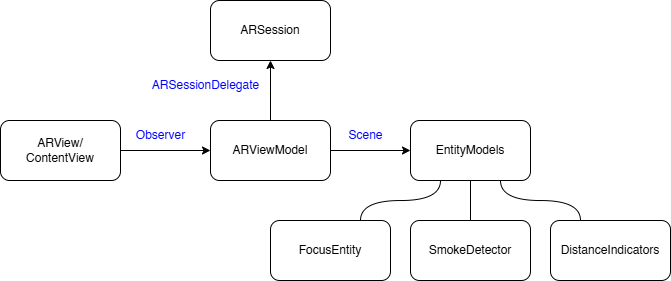
\includegraphics[width=0.8\textwidth]{Architecture}
    \caption{Softwarearchitektur des Prototypen}
    \label{fig:Architecture}
\end{figure}

Die View-Schicht ist für die Darstellung der Augmented-Reality-Szene und der UI-Elemente zuständig. Sie beobachtet das \texttt{ARViewModel} und aktualisiert die Anzeige basierend auf den empfangenen Daten. Das \texttt{ARViewModel} bildet die zentrale Steuerungseinheit der Anwendung. Es verwaltet die Kommunikation mit der \texttt{ARSession}, empfängt Tracking-Daten und verarbeitet Änderungen in der AR-Umgebung. Darüber hinaus aktualisiert es die Szene durch das Verwalten und Steuern der enthaltenen Augmented-Reality-Objekte.

Die AR-Objekte sind in der \texttt{EntityModels}-Komponente zusammengefasst. Diese beinhaltet verschiedene Entitäten, die in der Szene dargestellt werden, wie beispielsweise die \texttt{FocusEntity}, die als visuelle Markierung dient, um dem Nutzer eine Orientierung zu ermöglichen. Zudem enthält das System eine \texttt{SmokeDetector}-Entität, die zur Simulation oder Erkennung von Rauchmeldern verwendet werden kann, sowie \texttt{DistanceIndicators}, welche zur Visualisierung von Entfernungen innerhalb der Augmented-Reality-Szene genutzt werden.

Die Kommunikation zwischen diesen Komponenten erfolgt über ein \texttt{Observer}-Pattern. Dabei beobachtet die View das \texttt{ViewModel}, um Änderungen in der Szene dynamisch darzustellen. Mithilfe des Observation-Frameworks von Swift kann das Pattern einfach implementiert werden, ohne dass zusätzlicher Boilerplate-Code notwendig ist. Dazu muss die Klasse, die beobachtet werden soll, mit \texttt{@Observable} wie folgt annotiert werden:

\begin{lstlisting}[language=Swift]
@Observable
class ARViewModel {
    private(set) var scene: [Entity & HasAnchor] = []
    @ObservationIgnored private var isProcessing: Bool = false
    // ...
}
\end{lstlisting}

Sämtliche Änderungen an den Variablen werden automatisch an die beobachtenden Klassen weitergeleitet. Variablen, die nicht beobachtet werden sollen, können mit \texttt{@ObservationIgnored} annotiert werden. Dadurch wird eine effiziente und performante Kommunikation zwischen den Komponenten ermöglicht.

Das \texttt{ViewModel} empfängt kontinuierlich Daten von der \texttt{ARSession}. Dazu implementiert es das \texttt{ARSessionDelegate}-Protokoll, das Callback-Methoden bereitstellt, um auf Änderungen in der AR-Umgebung zu reagieren. Die \texttt{ARSession} ist für das Tracking der Umgebung und die Verarbeitung der Sensordaten zuständig. Sie liefert dem \texttt{ViewModel} Informationen über die Position und Orientierung der Kamera, erkannte Flächen und erkannte Objekte. Das \texttt{ViewModel} verarbeitet diese und gibt relevante Informationen an die \texttt{EntityModels} weiter. 

Die verwendete Architektur ermöglicht eine saubere Trennung der Verantwortlichkeiten und sorgt für eine effiziente Verwaltung der AR-Objekte. Gleichzeitig bleibt die Anwendung modular und erweiterbar, sodass neue Funktionen oder Entitäten problemlos integriert werden können.

\subsection{ARSession und ARView}

Die \texttt{ARSession} ist die zentrale Komponente des ARKit-Frameworks und bildet die Grundlage für die Entwicklung von Augmented-Reality-Anwendungen für mobile iOS-Geräte. Die Session wurde für den Prototypen wie folgt konfiguriert:

\begin{lstlisting}[language=Swift]
let config = ARWorldTrackingConfiguration()
config.planeDetection = [.horizontal, .vertical]
config.sceneReconstruction = .meshWithClassification
config.frameSemantics.insert(.sceneDepth)
\end{lstlisting}

Hier wird zunächst die Erkennung von sowohl horizontalen als auch vertikalen Flächen aktiviert. Diese Planes (Flächen) werden anhand der Kameradaten und der Tiefeninformationen des LiDAR-Sensors erkannt und setig optimiert beziehungsweise erweitert. Die Session stellt anhand der erkannten Flächen \texttt{ARPlaneAnchor}-Objekte zur Verfügung, die Informationen über die Position, Ausrichtung und Größe der Flächen enthalten. Mithilfe des RealityKit-Frameworks können diese Ankerpunkte genutzt werden, um virtuelle Objekte auf den Flächen zu platzieren.

Die Aktivierung der Szenenrekonstruktion unter der Verwendung von \texttt{.meshWithClassification} aktiviert die Rekonstruktion der Umgebung mithilfe der LiDAR-Daten. Dazu wird ein Mesh erzeugt, das die Oberflächen der Umgebung detailliert beschreibt. Dies ermöglicht eine präzise Platzierung von virtuellen Objekten und die exakte Bestimmung von Abständen und Größen. Zusätzlich stellt das Framework die Klassifizierung des Meshes zur Verfügung. Dabei verwendet ARKit die im Kapitel \ref{sec:SceneUnderstanding} beschriebene semantische Segmentierung, um die erkannten Flächen zu klassifizieren und zu unterscheiden. Die Klassifizierung umfasst folgende Kategorien:

\begin{lstlisting}[language=Swift]
    enum ARMeshClassification: Int {
        case ceiling
        case door
        case floor
        case none
        case seat
        case table  
        case wall
        case window
    }
\end{lstlisting}

Diese Klassifizierung bezieht sich nicht nur auf die segmentierten Meshes, sondern auch auf die einzelnen Faces, die die Meshes bilden. Dadurch kann die Anwendung die erkannten Flächen genauer analysieren und beispielsweise zwischen Wänden und Decken unterscheiden. Dies ist besonders wichtig für die Platzierung von virtuellen Objekten, da die Montageregeln spezifische Anforderungen an die Positionierung von Rauchmeldern vorgeben.

Das \texttt{ARModelView} kann, als Delegierter der ARSession, auf die verarbeitenden Daten in Form von \texttt{ARFrame}-Objekten zugreifen. Diese Informationen über das generierte Mesh, die erkannten Flächen und zusätzliche Tiefendaten. Das \texttt{ARModelView} verarbeitet diese Daten und ändert gegebenenfalls die Entitäten in der Szene. Die Klassifizierung der Meshes wird genutzt, um die abweichenden Abstände von speziellen Objekten, wie Türen oder Fenstern, zu berücksichtigen. Die Frame-Semantik \texttt{.sceneDepth} liefert zusätzliche Informationen über die Tiefeninformationen der Szene, die für die Platzierung von virtuellen Objekten verwendet werden können.

\subsection{Entitäten der AR-Szene}

Die Entitäten (Entities) der Augmented-Reality-Szene stellen die Model-Objekte des Prototypen dar. Dabei handelt es sich um virtuelle Objekte, die in der augmentierten Umgebung platziert werden und dem Benutzer eine visuelle Rückmeldung geben. Es wurde darauf geachtet, dass die Szene ein Minimum an visuellen Elementen enthält, um den Benutzer nicht zu überfordern. Wie in Abbildung \ref{fig:Architecture} dargestellt, beschränken sich die visualisierten Entitäten auf die folgenden Objekte:

\begin{itemize}
    \item \texttt{FocusEntity}
    \item \texttt{SmokeDetector}
    \item \texttt{DistanceIndicators}
\end{itemize}

Die Entitäten wurden so konzipiert, dass sie direkt in die Augmented-Reality-Szene platziert werden können und sich dynamisch an die Umgebung anpassen. Dazu wurden Protokolle und Klassen des \texttt{RealityKit}-Frameworks verwendet, die eine einfache Erstellung und Verwaltung von Augmented-Reality-Objekten ermöglichen. Im Beispiel der \texttt{SmokeDetector}-Entität wurde die Klasse wie folgt implementiert:

\begin{lstlisting}[language=Swift]
class SmokeDetector: Entity, HasModel, HasAnchoring {
    init() {
        super.init()
        // Initialization of MeshComponent and ModelComponent
    }
    // ...
}
\end{lstlisting}

Dabei wird die \texttt{SmokeDetector}-Entität als Subklasse der \texttt{Entity}-Klasse definiert. Die \texttt{Entity}-Klasse ist die Basisklasse für alle virutellen Objekte in der Augmented-Reality-Szene und stellt grundlegenden Funktionen zur Verfügung, um die Entitäten in der Szene zu verwalten. Die \texttt{SmokeDetector}-Entität implementiert das \texttt{HasModel}-Protokoll, das die Verwendung von 3D-Modellen in der Entität ermöglicht. Zusätzlich implementiert sie das \texttt{HasAnchoring}-Protokoll, das die Verankerung der Entität an einem AR-Anchor ermöglicht. Änderungen, die an der Entität vorgenommen werden, werden automatisch an die Augmented-Reality-Szene weitergeleitet und dort dargestellt.

Zugegeben, stellt die Verwendung von \texttt{RealityKit}-Komponenten in Model-Klassen eine Abhängigkeit zur View-Schicht dar. Eine strikte Trennung der Entity- und der Model-Klassen wäre wünschenswert, um die Wiederverwendbarkeit und Erweiterbarkeit der Model-Klassen zu gewährleisten. Dies würde aber eine zusätzliche Komplexität mit sich bringen und die Architektur unnötig verkomplizieren. Daher wurde im Rahmen des Prototypen entschieden, die \texttt{RealityKit}-Komponenten direkt in den Model-Klassen zu verwenden, um die Implementierung zu vereinfachen und die Entwicklung zu beschleunigen.

\subsection{Validierung der Montageregeln}

Die Implementierng der Montageregeln bilden, neben der Visualisierung, den Kern des Prototypen und sind Vorraussetzung für die korrekte Platzierung der Rauchmelder. Aus diesem Grund ist es wichtig, dass die Regeln korrekt und zuverlässig umgesetzt werden und einfach erweiterbar sind. Für den Prototypen wurden Mindestanforderungen bezüglich der im Kapitel \ref{cha:Problemstellung} beschriebenen Regeln definiert. Diese Mindestanforderungen umfassen die folgenden Regeln:

\begin{itemize}
    \item Der Rauchmelder darf nur an Decken montiert werden
    \item Der Rauchmelder muss mindestens 50 cm von Wänden entfernt sein
    \item Der Rauchmelder muss mindestens 1,50 m von Türen und Fenstern entfernt sein
\end{itemize}

Dazu wurde ein Framework entwickelt, das die Validierung der Montageregeln übernimmt. Zentrale Komponente des Frameworks ist der \texttt{MountingRuleManager}. Diese Klasse verwaltet eine Liste von Montageregeln. 

Diese Regeln sind als Klassen implementiert und implementieren das \texttt{MountingRule}-Protokoll. Das Protokoll definiert eine Funktion, die die Validierung der Regel durchführt und einen booleschen Wert zurückgibt:

\begin{lstlisting}[language=Swift]
protocol MountingRule {
    var errorType: MountingErrorType { get }
    func validateRule(for focus: ARRaycastResult, in session: ARSession) async -> Bool
}
\end{lstlisting}


Zusätzlich dazu wird ein \texttt{MountingErrorType} angegeben, der den Typ des Fehlers angibt, falls die Regel nicht erfüllt ist. Entsprechend der zuvor beschriebenen Mindestanforderungen wurden folgende \texttt{MountingErrorType}-Werte definiert:

\begin{lstlisting}[language=Swift]
enum MountingErrorType {
    case ceilingRuleError
    case wallRuleError
    case windowOrDoorRuleError
    case none
}
\end{lstlisting}

Abhängig von diesem Typ wird der Status der virtuelle Montage angepasst und dem Benutzer eine entsprechende Rückmeldung gegeben. 

Der \texttt{MountingRuleManager} stellt eine Funktion zur Verfügung, welche die Validierung der gegebenen Regeln ausführt und den Status der Montage zurückgibt:


\begin{lstlisting}[language=Swift]
class MountingRuleManager {
    private var rules: [MountingRule] = []
    
    // Initializer
    
    func validateRules(for focus: ARRaycastResult, in arSession: ARSession) async -> errorType: MountingErrorType {
        for rule in rules {
            if await !rule.validateRule(for: focus, in: arSession) {
                return rule.errorType
            }
        }
        return .none
    }
}
\end{lstlisting}

Die Funktion iteriert über die Liste der Regeln und führt die Validierung für jede Regel aus. Falls eine Regel nicht erfüllt ist, wird der entsprechende \texttt{MountingErrorType} zurückgegeben. Andernfalls wird \texttt{.none} zurückgegeben, um anzuzeigen, dass alle Regeln erfüllt sind.

Der \texttt{MountingRuleManager} wird im \texttt{ARViewModel} initialisiert und verwendet. Dabei ist die Reihenfolge der Regeln entscheidend, da die Regeln nacheinander überprüft werden. Für den Prototypen wurde die Reihenfolge der Regeln so gewählt, dass die wichtigsten Regeln zuerst überprüft werden. Dies ermöglicht eine effiziente Überprüfung der Regeln und eine schnelle Rückmeldung an den Benutzer.

Die beschriebene Implementierung stellt eine einfache und leicht erweiterbare Lösung dar, um die Montageregeln zu validieren und dem Benutzer eine Rückmeldung zu geben. Die Regeln können einfach hinzugefügt oder geändert werden, um neue Anforderungen zu berücksichtigen oder bestehende Regeln zu optimieren.

\subsection{FocusEntity}

\subsection{Performance-Optimierung}
Wie in den Anforderungen beschrieben, spielt die Performance eine entscheidende Rolle bei der Entwicklung von Augmented-Reality-Anwendungen. Sie wird von verschiedenen Faktoren beeinflusst, darunter die Verarbeitungsgeschwindigkeit der Sensordaten, die Darstellung virtueller Objekte und die Interaktion mit dem Benutzer. Um eine hohe Performance sicherzustellen, wurden gezielte Optimierungsmaßnahmen implementiert, die die Datenverarbeitung effizienter gestalten und die Darstellung der AR-Szene beschleunigen.

Bevor Multithreading als Optimierungsstrategie in Betracht gezogen wurde, lag der Fokus darauf, die synchrone Implementierung zu verbessern. Dabei wurden drei zentrale Aspekte identifiziert:

\begin{itemize}
\item Reduktion der Verarbeitungsfrequenz der ARFrame-Daten
\item Optimierung der Raycast-Abstandsprüfung
\item Filterung der ARMeshAnchors zur effizienteren Abstandsanalyse
\end{itemize}

Die Verarbeitung der ARFrame-Daten wurde optimiert, indem die Regelprüfung nur noch alle 10 Frames durchgeführt wird. Dies reduziert die Anzahl der Berechnungen erheblich und steigert die Verarbeitungsgeschwindigkeit.

Die Anzahl der Raycasts zur Abstandskontrolle wurde von 30 auf 9 gesenkt. Dadurch wird der Rechenaufwand weiter verringert, was zu einer spürbaren Effizienzsteigerung bei der Überprüfung von Abständen führt.

Zusätzlich erfolgt bei der Analyse der ARMeshAnchors nun eine Vorabfilterung: Anker, die sich außerhalb des Mindestabstands zu Türen und Fenstern befinden, werden direkt ausgeschlossen. Dies reduziert die Anzahl der zu überprüfenden Anker signifikant und beschleunigt die Abstandskontrolle.

Dank dieser Maßnahmen konnte die Performance der Anwendung deutlich verbessert werden, ohne dass zunächst auf parallele Verarbeitung zurückgegriffen werden musste.

Im nächsten Schritt wurde die Implementierung von Multithreading in Betracht gezogen, um die Verarbeitung der ARFrame-Daten weiter zu beschleunigen. Dabei wurde auf das async/await-Feature von Swift zurückgegriffen, das eine einfache und effiziente Implementierung von asynchronen Operationen ermöglicht. Die Funktionen zur Überprüfung der Montageregeln wurden in einen separaten Thread ausgelagert, um die Hauptverarbeitungsschleife und somit die ARView nicht zu blockieren. Dadurch wird die Reaktionszeit der Anwendung verbessert und die Performance insgesamt gesteigert.

\subsection{Raycasting} \label{Raycasting}
 

\textit{Raycasting} ist eine Technik, die in der Computergrafik und in Augmented-Reality-Systemen weit verbreitet ist. Sie wird zum Beispiel verwendet, um die Sichtlinie eines Benutzers zu simulieren und zu überprüfen, ob sie ein bestimmtes Objekt trifft. Die Abbildung \ref{fig:Raycasting} zeigt die Funktionsweise des \textit{Raycastings}. Bei dieser Technik wird ein Strahl (\textit{Ray}) von einem Startpunkt in eine bestimmte Richtung geschossen und geprüft, ob er ein Objekt trifft.

\begin{figure}[ht]
    \centering
    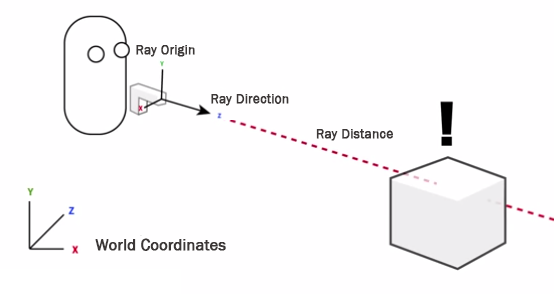
\includegraphics[width=0.8\textwidth]{Raycast}
    \caption{Funktionsweise des \textit{Raycastings}}
    \label{fig:Raycasting}
\end{figure}

Das ARKit-Framework stellt eine Funktion zur Verfügung, um \textit{Raycasts} in der AR-Szene durchzuführen. Hierbei lässt sich der Startpunkt und die Richtung des Strahls mithilfe eines \texttt{RaycastQuery}-Objekts definieren. Die Funktion liefert ein Array von \texttt{ARRaycastResult}-Objekten zurück, die Informationen über die Position der Schnittpunkte mit den getroffen Zielen, die Art der getroffenen Ziele und die Orientierung dessen. Falls es sich bei dem getroffenen Ziel einen \texttt{ARAnchor} besitzt, wird dieser ebenfalls zurückgegeben.

Mithilfe von \textit{Raycasts} wurde die Validierung des Mindestabstandes zu umgebenen Wänden implementiert. Um die Umgebung auf zu nahen Wänden zu überprüfen, werden mehrere \textit{Raycasts} in einem 360-Grad-Winkel parallel zur x-z-Ebene um die Fokus-Entität durchgeführt. Trifft der Strahl auf ein Objekt, wird davon ausgegangen, dass es sich bei diesem um eine Wand bieziehungsweise ein Objekt, welches eine Wand darstellt, handelt. Anschließend wird der Abstand von diesem Objekt zur Fokus-Entität berechnet und mit dem vordefinierten Mindestabstand verglichen. Unterschreitet die Distanz den Mindestabstand, wird die Position der Fokus-Entität als ungültig angesehen und die Montage des virtuellen Rauchmelders verhindert.

Zusätzlich dazu stellt das \textit{Raycasting} die Grundlage der Positionierung der Fokus-Entität dar. Dabei wird bei jedem Frame ein Raycast von der Kamera in das Zentrum der Augmented-Reality-Szene geschossen und die Position des ersten getroffenen Objekts als Position der Fokus-Entität verwendet. Dies ermöglicht eine präzise Platzierung der Fokus-Entität und eine genaue Ausrichtung des virtuellen Rauchmelders.

\subsection{View}

Die View des Prototypen wurde mithilfe des SwiftUI-Frameworks von Apple implementiert. Diese Framework verwendet eine deklarative Syntax, um Benutzeroberflächen zu erstellen und zu verwalten. Dabei stellen einzelne \texttt{View}-Komponenten die Bausteine der Benutzeroberfläche dar, die mithilfe von Modifikatoren und Containern zu komplexen Layouts zusammengesetzt werden können. Der komponentenbasierte Aufbau der Benutzeroberfläche kann gut als Baumstruktur dargestellt werden:

\begin{figure}[h]
    \centering
    \begin{minipage}{0.45\textwidth}
        \centering
        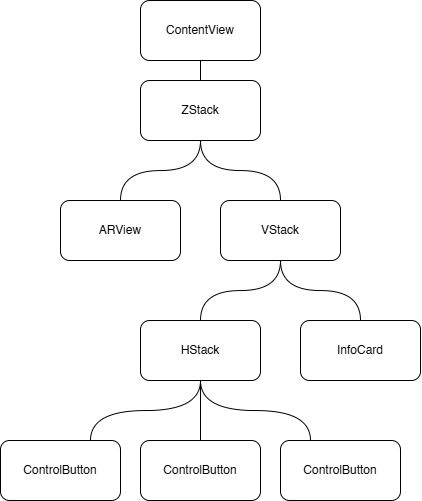
\includegraphics[width=\textwidth]{UI}
        \label{fig:UITree}
    \end{minipage}
    \hfill
    \begin{minipage}{0.45\textwidth}
        \centering
        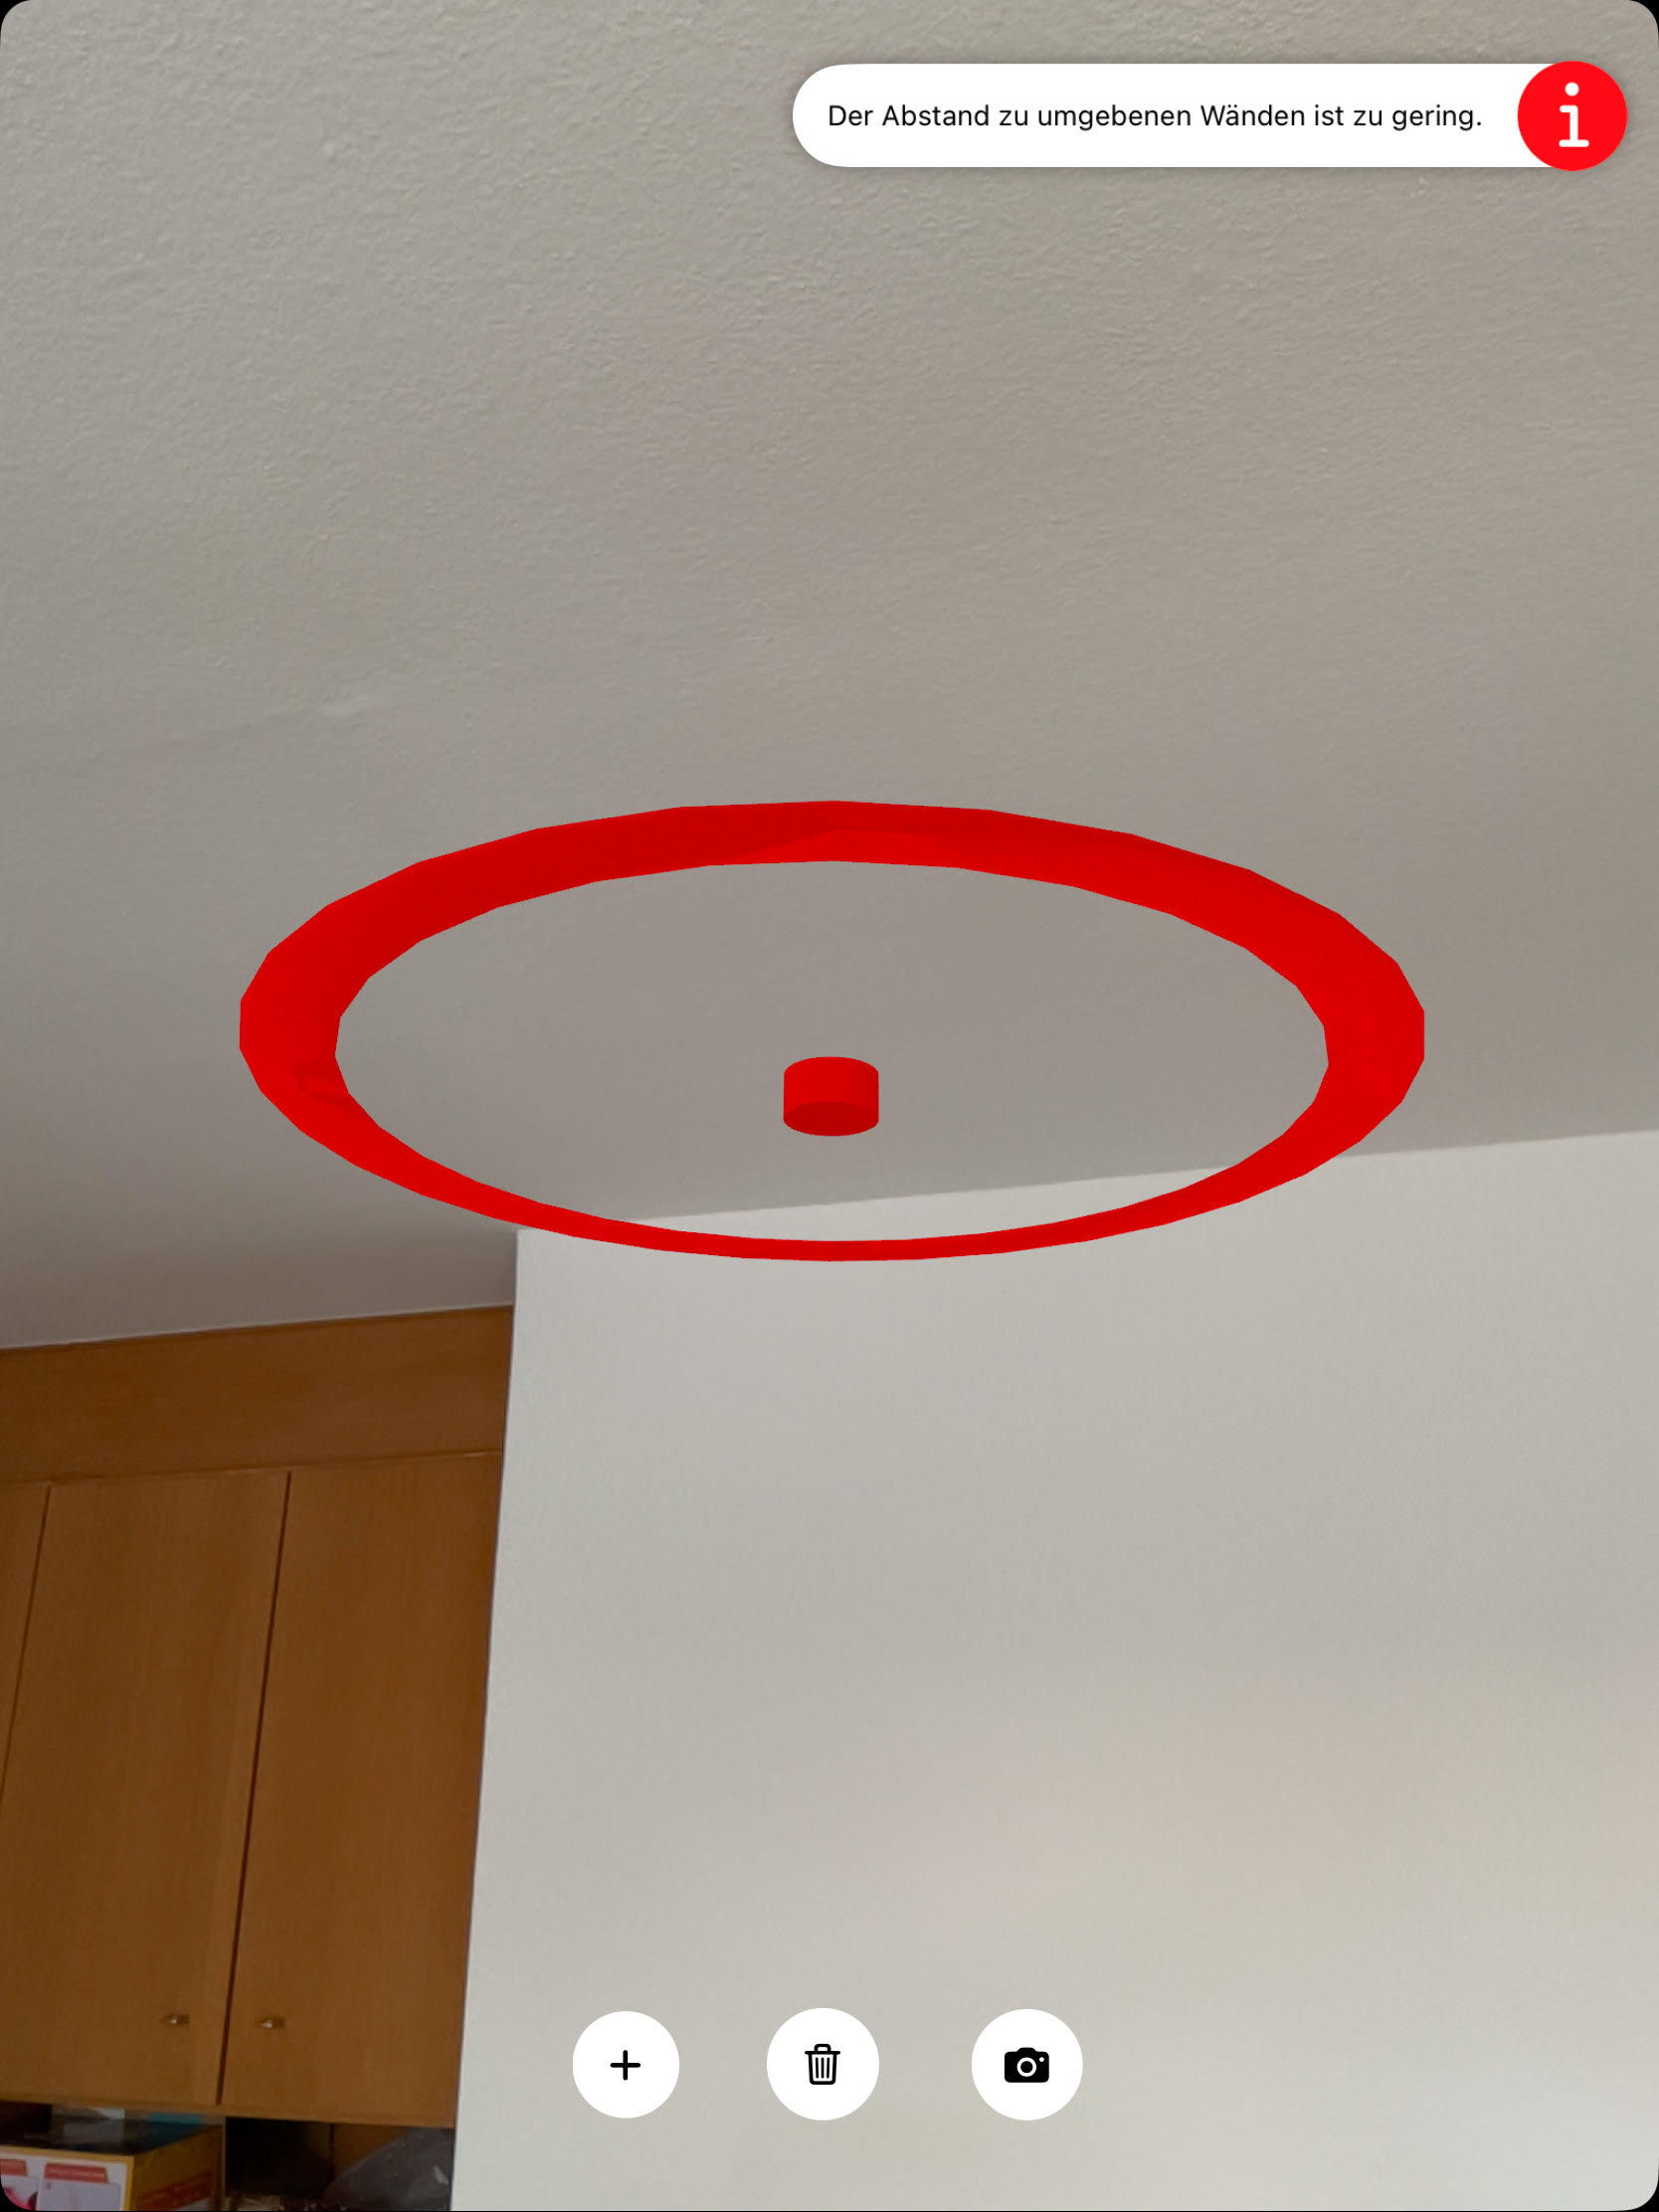
\includegraphics[width=\textwidth]{AppUI}
        \label{fig:UIApp}
    \end{minipage}
    \caption{SwiftUI-Benutzeroberfläche: Baumstruktur (links) und App-Ansicht (rechts)}
\end{figure}

Dieser Aufbau ermöglicht eine übersichtliche Implementierung der Benutzeroberfläche und eine einfache Anpassung der einzelnen Komponenten. Die Komponenten können so implementiert werden, dass sie unabhängig voneinander sind und wiederverwendet werden können. So wird der \texttt{ControlButton} beispielsweise mehrfach mit unterschiedlichen Icons und Callback-Funktionen verwendet.

\begin{lstlisting}[language=Swift]
struct ControlButton: View {
    var iconName: String
    var action: () -> Void
        
    var body: some View {
        // Implementatierung der Button-Komponente
    }
}
\end{lstlisting}

SWiftUI stellt eine Vielzahl von vordefinierten Komponenten zur Verfügung, die für die Entwicklung von iOS-Anwendungen optimiert sind. So wird beispielsweise die \texttt{ZStack}-Komponente verwendet, um die Buttons und die InfoCard über der ARView zu legen. 

Zusätzlich dazu wurden Modifikatoren verwendet um die Darstellung der Komponenten zu steuern. So wurden beispielsweise Übergänge und Animationen definiert, um die Zustandsänderungen der \texttt{InfoCard} zu visualisieren:

\begin{lstlisting}[language=Swift]
InfoText(infoText: infoText)
    .transition(.move(edge: .trailing))
    .animation(.easeInOut(duration: 0.5), value: infoText)
    .opacity(infoText.isEmpty ? 0 : 1)
    .animation(.easeInOut(duration: 0.4), value: infoText)
\end{lstlisting}

Der \texttt{transition}-Modifikator stellt eine Bewegung der Komponent von der rechten Bildschirmkante dar. Diese Bewegung wird mithilfe des \texttt{animation}-Modifikators animiert. Um den Übergangseffekt zu verstärken wurde außerdem ein \texttt{opacity}-Modifikator animiert, der den Übergang der Transparenz der Komponente darstellt. 

Die ARView stellt die Rendering-Engine für die Augmented-Reality-Szene dar. Sie ist Teil des RealityKit-Frameworks und ermöglicht die Darstellung von 3D-Objekten in einer augmentierten Umgebung. Damit die ARView in die SwiftUI-View integriert werden kann, muss sie als \texttt{UIViewRepresentable}-Komponente eingebunden werden. Dabei wird die ARView als Subview der SwiftUI-View hinzugefügt und mithilfe von Modifikatoren positioniert und skaliert. 


[X] Architektur: Struktur, Programmablauf, MVVM

[ ] Session: Setup/Initialisierung/Daten

[X] ViewModel: Raycasting, isPlaceable

[ ] RealityKid-Entities: FocusEntity, SmokeDetector, DistanceIndicators

[ ] FocusEntity gesondert: Implementierung

[X] Performance: Multi-Threading, Single Processing, Processing Frequency

[X] Views: ARView und SwiftUI

Der Zustand gibt an, ob die implementierten Mindestanforderungen erfüllt sind oder nicht. Dabei erfolgt die Überprüfung der Regeln schrittweise. Zunächst wird geprüft, ob die Focus-Entity aktuell auf eine Decke zeigt. Dazu wird im ersten Schritt überprüft ob die Entität mit einem \texttt{ARPlaneAnchor} verankert ist. Anschließend wird die Klassifizierung des Ankers überprüft, um festzustellen, ob es sich um eine Decke handelt. Ist dies nicht der Fall, wird der Zustand auf \texttt{notOnCeiling} gesetzt.

Im nächsten Schritt werden die Abstände zu den Wänden geprüft. Es wurden zwei unterschiedliche Ansätze für die Überprüfung der Abstände zu umliegenden Wänden in Erwägung gezogen. Der erste Ansatz basiert auf dem Collision-Detection-System von RealityKit, das die Kollisionen zwischen den AR-Objekten erkennt. Dazu würde eine unsichtbare oder transparente Kugel mit einem Radius, der dem Mindestabstand zu den Wänden entpsricht, um die Fokus-Entität platziert werden, die die Kollisionen mit den Wänden überprüft. Falls eine Kollision mit einem \texttt{ARPlaneAnchor} erkannt wird, wird der Zustand auf \texttt{constraintsNeglected} gesetzt. 

Der zweite Ansatz basiert auf dem in \ref{Raycasting} beschriebenen Raycast-Verfahren. Um die Umgebung auf zu nahen Wänden zu überprüfen, werden mehrere Raycasts in einem 360-Grad-Winkel parallel zu x-z-Ebene um die Fokus-Entität durchgeführt. Trifft der Raycast auf einen \texttt{ARPlaneAnchor} mit der Alignment-Eigenschaft \texttt{.vertical}, wird der Abstand zur Fokus-Entität berechnet. Dabei wird die Distanz mithilfe der Positionen der Fokus-Entität berechnet und mit dem Mindestabstand verglichen. Unterschreitet die Distanz den Mindestabstand, wird der Zustand auf \texttt{constraintsNeglected} gesetzt.

Recherchen bezüglich beider Ansätze lässt darauf schließen, dass die Berechnung der Distanz mithilfe von Raycasts performter ist als die Kollisionserkennung. Daher wurde der zweite Ansatz für die Überprüfung der Abstände verwendet.

Im letzten Schritt werden die Abstände zu Türen und Fenstern überprüft. Dazu werden \texttt{ARMeshAnchor} im \texttt{ARFrame} analysiert. Diese ARMeshAnchor entsprechen physikalischen Objekten in der Umgebung, die mithilfe der LiDAR-Daten erkannt wurden und mit einem polygonalen Mesh beschrieben werden. Diese Daten werden wie folgt analysiert:

\begin{lstlisting}[language=Swift]
for anchor in frame.anchors.compactMap({ $0 as? ARMeshAnchor }) {
    for index in 0..<anchor.geometry.faces.count {
        if [.window, .door].contains(anchor.geometry.classificationOf(faceWithIndex: index)),
           distance(anchor.geometry.centerOf(faceWithIndex: index), focusEntity.position) < MountingRules.minDistanceToWindowsAndDoors {
            state = .constraintsNeglected
            return
        }
    }
}
\end{lstlisting}

Zunächst werden mithilfe der \texttt{compactMap()}-Funktion alle Anker aus dem \texttt{ARFrame} entfernt, die nicht vom Typ \texttt{ARMeshAnchor} sind. Anschließend werden die verbleibenden Anker in einer \texttt{for}-Schleife analysiert, um die Klassifizierung des Meshes zu überprüfen. Dabei wird für jedes Face des Meshes die Klassifizierung abgefragt und geprüft, ob es sich um eine Tür oder ein Fenster handelt. Trifft dies zu, wird der Abstand zur Fokus-Entität berechnet und mit dem Mindestabstand verglichen. Unterschreitet die Distanz den Mindestabstand, wird der Zustand auf \texttt{constraintsNeglected} gesetzt.

Erst wenn die Überprüfung der Regeln vollständig abgeschlossen ist und alle Anforderungen erfüllt sind, wird der Zustand auf \texttt{constraintsSatisfied} gesetzt und die Montage des virtuellen Rauchmelders kann erfolgen.
